\subsection{Forward Stepwise Selection}

The first method applied is the \textit{Forward Stepwise Selection}. In particural, the algorithm variant employed uses the \textit{p-value} a entrance criterion and the AIC as comparison metric between models. The model obtained is shown in figure \Fig~\ref{fig:ForwardModelSummary}.
\begin{figure}[h]
	\centering
	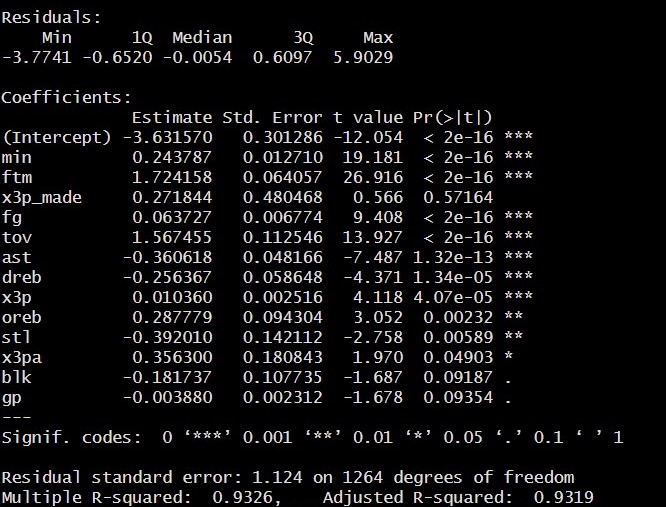
\includegraphics[width=0.4\linewidth]{ImageFiles/Regression/Forward/ForwardModelSummary}
	\caption{Forward Stepwise Selection Output Model.}
	\label{fig:ForwardModelSummary}
\end{figure}

As expected \textit{"MIN"} is included and also \textit{"FTM"} which resulted to be important from the preliminary analysis. However, there are three variables that are not significantly different from 0, with p-value threshold of $5\%$.

\vspace{0.2cm}
\textbf{Bootstrap Statistical Inference}

On the obtained model we the \textit{Bootstrap} technique in order to perform statistical inference over the model coefficients. In figure \Fig~\ref{fig:ForwardModelSummary} is possible to see the results, that are coherent with the previous ones. This shows also that the Gaussian approximation is valid in this case.
\begin{figure}[h]
	\centering
	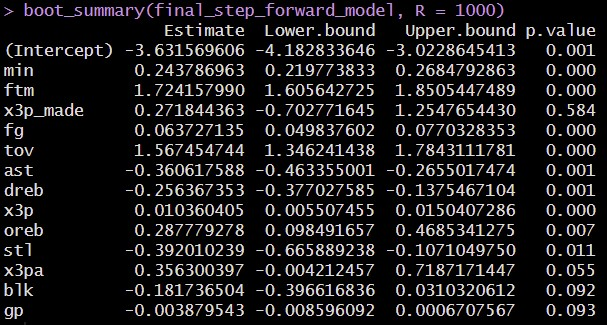
\includegraphics[width=0.4\linewidth]{ImageFiles/Regression/Forward/BootForwardModel}
	\caption{Boostrap results on Forward Stepwise Selection Output Model.}
	\label{fig:BootForwardModel}
\end{figure}

\vspace{0.2cm}
\textbf{Final Forward Model}

The final Forward Model, shown in figure \Fig~\ref{fig:ForwardFinalModelSummary}, is obtained removing the non significant variables. In \Fig~\ref{fig:ForwardFinalModelResiduals} and \Fig~\ref{ForwardFinalModelResidualsDist} instead is possible to see plot of the residuals, that have a Gaussian shape with 0 mean. This means that the model is likely good enough.

\begin{figure}[h]
	\centering
	\begin{subfigure}{.6\textwidth}
		\centering
		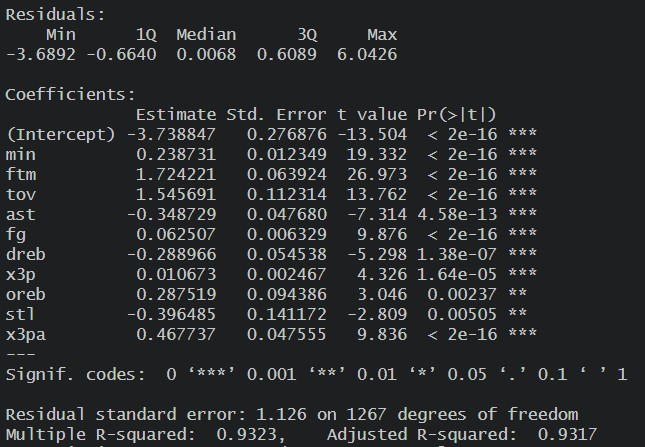
\includegraphics[width=0.6\linewidth]{ImageFiles/Regression/Forward/ForwardFinalModelSummary}
		\caption{Forward Stepwise Selection Model Summary.}
		\label{fig:ForwardFinalModelSummary}
	\end{subfigure}
	\begin{subfigure}{.6\textwidth}
		\centering
		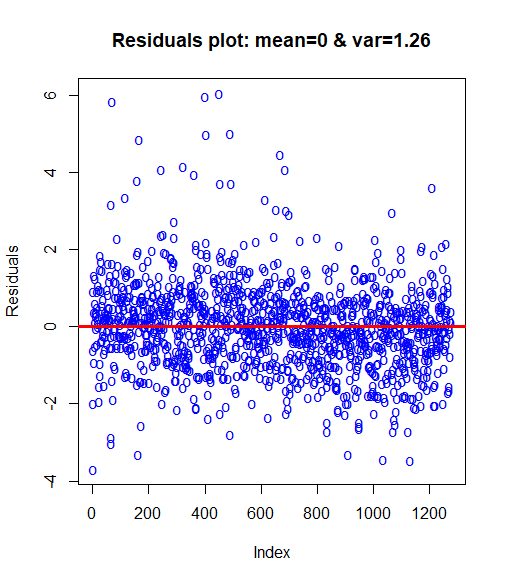
\includegraphics[width=0.6\linewidth]{ImageFiles/Regression/Forward/ForwardFinalModelResiduals}
		\caption{Forward Stepwise Selection Model Residuals.}
		\label{fig:ForwardFinalModelResiduals}
	\end{subfigure}%
	\begin{subfigure}{.6\textwidth}
		\centering
		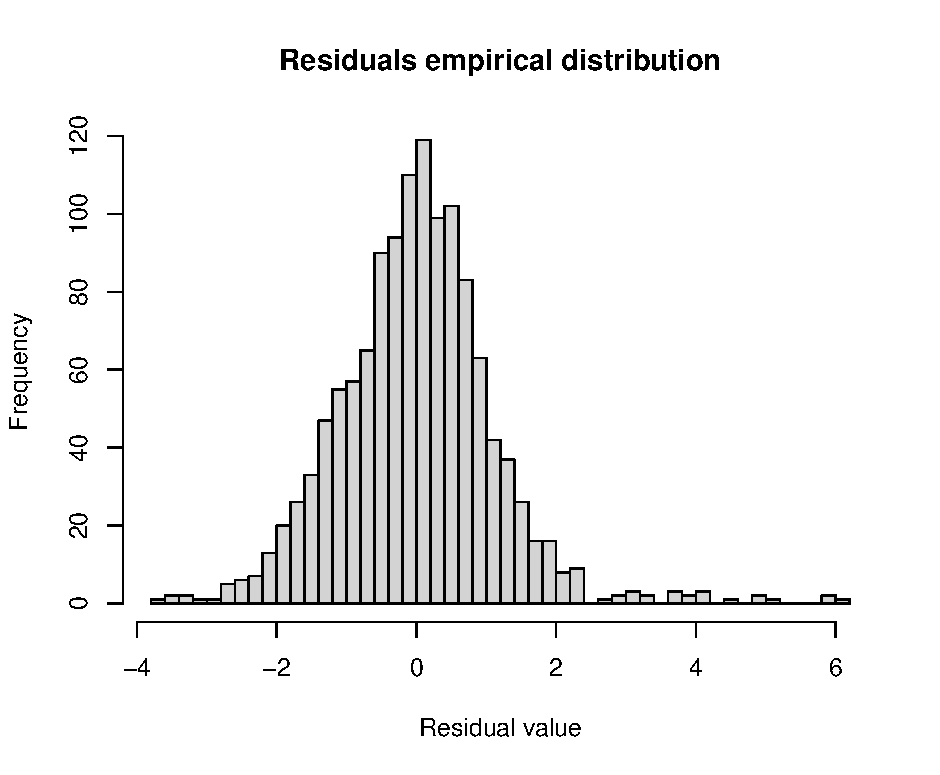
\includegraphics[width=0.6\linewidth]{ImageFiles/Regression/Forward/ForwardFinalModelResidualsDist}
		\caption{Forward Stepwise Selection Model Residuals.}
		\label{fig:ForwardFinalModelResidualsDist}
	\end{subfigure}
\end{figure}

